Esta sección aborda la fase de despliegue de los modelos de clasificación binaria y multiclase desarrollados para la detección de conexiones malignas. La fase de despliegue en la metodología CRISP-DM implica la integración de los modelos entrenados en entornos operativos donde sus predicciones contribuyen a la toma de decisiones en tiempo real o en análisis periódicos, facilitando la detección automatizada y escalable de amenazas en redes como se comenta en capítulos anteriores \cite{wirth2000crisp}.

\section{Integración en entornos operativos}

Los modelos de clasificación binaria, orientados a distinguir conexiones malignas de benignas, y los modelos multiclase, diseñados para identificar diferentes categorías de conexiones malignas, deben ser implementados en plataformas que permitan la recepción continua de datos y procesamiento eficiente \cite{baylor2017tensorflow}. 

Para ello, es recomendable desplegarlos mediante APIs o microservicios, asegurando compatibilidad con sistemas de monitorización y respuesta automatizada. En el caso del modelo multiclase, la alta desproporción entre las clases y la naturaleza específica de los datos requieren especial atención en la validación en entorno real, dado que durante la fase de evaluación correspondiente con el capítulo \ref{cap.test} se utiliza el conjunto completo de datos y puede observarse degradación en desempeño frente a la fase de búsqueda \cite{gama2014survey}.

\section{Consideraciones técnicas}

El uso de validación cruzada estratificada durante la fase de búsqueda garantiza la estabilidad en la estimación de rendimiento, pero el despliegue debe contemplar la variabilidad inherente a datos nuevos y no vistos, especialmente en contextos dinámicos como la detección de conexiones malignas \cite{reimers2017optimal}. 

El ajuste adecuado de hiperparámetros, demostrado durante el capítulo \ref{cap.modelos}, debe ser preservado en producción, considerando limitaciones de hardware, latencia y volumen de datos. El control de versiones de los modelos es crucial para realizar actualizaciones y retrocesos en sus configuraciones de pesos, sin afectar a los resultados que devuelva el modelo \cite{peters2017machine}.

\subsection{Patrones arquitectónicos recomendados: Pipeline y Observador}

Para garantizar un despliegue robusto y adaptable de los modelos de clasificación en entornos operativos, lo recomendable es estructurar el sistema empleando patrones arquitectónicos que favorezcan la modularidad, la escalabilidad y la capacidad de respuesta ante eventos. Los patrones \textit{Pipeline} o Filtro Tuberia y Observador destacan como enfoques adecuados para satisfacer los requerimientos funcionales y no funcionales del sistema.

El patrón \textit{Pipeline} permite organizar el procesamiento de datos en una secuencia de etapas independientes, donde cada etapa representa una transformación o acción específica sobre el flujo de datos. Este enfoque favorece la separación de responsabilidades, facilita el mantenimiento, y permite escalar individualmente cada componente. Es particularmente útil para el procesamiento continuo de datos en tiempo real, como en entornos de detección de conexiones malignas \cite{neptune_ml_pipeline}.

Por otro lado, el patrón Observador resulta útil para implementar una arquitectura reactiva, en la cual distintos componentes del sistema (por ejemplo, sistemas de alerta, interfaces de usuario, módulos de registro) pueden suscribirse a los eventos generados por el modelo como la detección de una amenaza. Este patrón facilita una integración flexible entre los modelos de predicción y otros servicios que requieren actuar en función de los resultados generados, sin acoplamiento directo entre ellos \cite{gof_observer_pattern}.

La combinación de ambos patrones permite un diseño desacoplado, extensible y más mantenible, características fundamentales para sistemas de monitorización y respuesta en entornos dinámicos y críticos como la ciberseguridad.


\section{Monitorización y mantenimiento}
Una vez desplegados, los modelos requieren monitorización continua para detectar posibles cambios en la distribución de los datos o en el comportamiento de las conexiones, que puedan afectar el rendimiento del modelo (\textit{data drift} y \textit{concept drift}) \cite{gama2014survey}. En particular, para el modelo multiclase que ha sido entrenado con clases muy desbalanceadas, la monitorización de métricas como el \textit{F1-Weighted} es esencial para asegurar la calidad del diagnóstico en todas las categorías.

El mantenimiento de los modelos, incluye la recopilación de datos reales etiquetados, la reevaluación periódica del modelo y la posible reentrenamiento o ajuste de hiperparámetros para mantener la eficacia en la detección \cite{tsymbal2004problem}.

\section{Impacto y aplicación en el mundo real}

El despliegue efectivo de estos modelos contribuye a mejorar la seguridad en redes mediante la automatización de la detección de conexiones malignas, permitiendo respuestas rápidas y reducción de falsos positivos y negativos. La diferenciación entre múltiples tipos de conexiones malignas aporta un valor añadido para estrategias de mitigación específicas y optimización de recursos \cite{amershi2019software}.

La Figura \ref{fig:despliegue} muestra como podría implementarse de manera básica los modelos desarrollados en un entorno real de un sistema informático.

\begin{figure}[H]
    \centering
    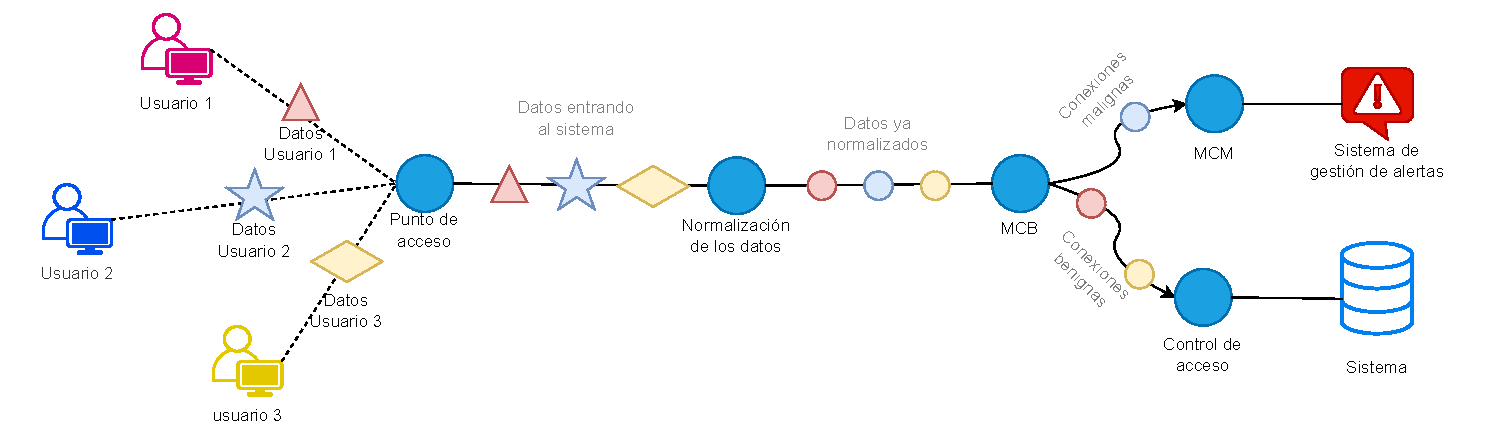
\includegraphics[width=1\textwidth]{./img/despliegue/despliegue.pdf}
    \caption{Ejemplo de despliegue de los modelos en un sistema informático.}
    \label{fig:despliegue}
\end{figure}
